\documentclass[10pt]{beamer}
\usepackage[T2A]{fontenc}       %поддержка кириллицы
\usepackage[utf8]{inputenc}
\usepackage{lmodern}
\usepackage{scrextend}
\changefontsizes{16pt}
\usepackage{listings}
\usepackage{xcolor}
\graphicspath{{./images/}}
\usetheme{default}
\usecolortheme{crane}
\usefonttheme{structurebold}
\usefonttheme[onlymath]{serif}
\setbeamercovered{transparent}
\definecolor{name}{rgb}{0.5,0.5,0.5}
\begin{frame}{PHP}
  \begin{center}
    \begin{itemize}
      \item Interpretation
      \item Dynamic typing
      \item Garbage collector
      \item Procedure \& OOP
    \end{itemize}
  \end{center}
\end{frame}

\title[Web]{Web программирование}
\subtitle[HTTP]{HyperText Transfer Protocol}
\author[Родионов И.Н.]{Игорь Родионов}
\institute[ОмГТУ ИВТ]{Омский Государственный Технический Университет\\
	{\tiny кафедра Информатики и вычислительной техники}\\
}
\date[2014]{ОмГТУ, 2014.}

\begin{document}
\begin{frame}[plain]
\maketitle
\end{frame}

\begin{frame}{Main Rule}
  \LARGE
  \begin{center}
    НЕ ДОВЕРЯЙТЕ ВХОДНЫМ ДАННЫМ
  \end{center}
\end{frame}
\begin{frame}{HTTP - Request (Запрос)}
GET /wiki/страница HTTP/1.1 \newline
Host: ru.wikipedia.org \newline
User-Agent: MyLonelyBrowser/5.0 \newline
Accept: text/html \newline
Connection: close \newline
\newline
\end{frame}
\begin{frame}{HTTP - Request methods}
    \begin{columns}[t] % contents are top vertically aligned
         \begin{column}[T]{5cm} % each column can also be its own environment
            \begin{center}
                \textbf{Idempotence}
                 \begin{itemize}
                     \item GET
                     \item HEAD
                 \end{itemize}
            \end{center}
         \end{column}
         \begin{column}[T]{5cm} % alternative top-align that's better for graphics
            \begin{center}
                \textbf{Non-idempotence}
                 \begin{itemize}
                     \item POST
                 \end{itemize}
             \end{center}
         \end{column}
     \end{columns}
\end{frame}


\begin{frame}{HTTP - Request methods}
    \begin{columns}[t] % contents are top vertically aligned
         \begin{column}[T]{5cm} % each column can also be its own environment
            \begin{center}
                 \begin{itemize}
                     \item PUT
                     \item PATCH
                     \item DELETE
                     \item OPTIONS
                 \end{itemize}
            \end{center}
         \end{column}
         \begin{column}[T]{5cm} % alternative top-align that's better for graphics
            \begin{center}
                 \begin{itemize}
                     \item LINK
                     \item UNLINK
                     \item CONNECT
                     \item TRACE
                 \end{itemize}
             \end{center}
         \end{column}
     \end{columns}
 \end{frame}

\include{sources/pages/http/methods_save}
\include{sources/pages/http/methods_idempotent} % check english wikipedia
\begin{frame}{HTTP - Request (Запрос)}
GET /wiki/страница HTTP/1.1 \newline
Host: ru.wikipedia.org \newline
User-Agent: MyLonelyBrowser/5.0 \newline
Accept: text/html \newline
Connection: close \newline
\newline
\end{frame}
\begin{frame}{HTTP - Response (Ответ)}
HTTP/1.1 200 OK \newline
Date: Wed, 11 Feb 2009 11:20:59 GMT \newline
X-Powered-By: PHP/5.2.4-2ubuntu5wm1\newline
Content-Type: text/html; charset=utf-8\newline
Content-Length: 1234\newline
Connection: close\newline
(пустая строка)\newline
(далее следует запрошенная страница в HTML)\newline
\newline
\end{frame}
\begin{frame}{HTTP - Response status codes}
            \begin{center}
                 \begin{itemize}
                     \item 1xx Informational (информационные)
                     \item 2xx Success (успешно)
                     \item 3xx Redirection (перенаправление)
                     \item 4xx Client Error (ошибка клиента)
                     \item 5xx Server Error (ошибка сервера)
                 \end{itemize}
            \end{center}
\end{frame}

\begin{frame}{HTTP - Response status codes}
            \begin{center}
                 \begin{itemize}
                     \item 200 OK
                     \item 301 Moved Permanently
                     \item 302 Moved Temporarily
                     \item 307 Temporary Redirect
                 \end{itemize}
            \end{center}
\end{frame}

\begin{frame}{HTTP - Response status codes}
            \begin{center}
                 \begin{itemize}
                     \item 403 Forbidden
                     \item 404 Not Found
                     \item 418 I'm a teapot
                     \item 500 Internal Server Error
                     \item 503 Service Unavailable
                     \item 504 Gateway Timeout
                 \end{itemize}
            \end{center}
\end{frame}
\begin{frame}{HTTP - Response (Ответ)}
HTTP/1.1 200 OK \newline
Date: Wed, 11 Feb 2009 11:20:59 GMT \newline
X-Powered-By: PHP/5.2.4-2ubuntu5wm1\newline
Content-Type: text/html; charset=utf-8\newline
Content-Length: 1234\newline
Connection: close\newline
(пустая строка)\newline
(далее следует запрошенная страница в HTML)\newline
\newline
\end{frame}
\begin{frame}{HTTP - Headers}
  Content-Disposition: form-data; name="AttachedFile1"\newline
  \newline
  Accept: text/plain\newline
  Accept-Charset: utf-8\newline
  Content-Range: bytes 88080384-160993791/160993792\newline
  \newline
  Content-Type: text/html;charset=utf-8\newline
  Location: http:\/\/example.com\/about.html\newline
\end{frame}
\begin{frame}{HTTP}
    \begin{columns}[t] % contents are top vertically aligned
         \begin{column}[T]{6cm} % each column can also be its own environment
            \begin{center}
                \textbf{Преимущества}
                 \begin{itemize}
                     \item Простота
                     \item Расширяемость
                     \item Распространённость
                 \end{itemize}
            \end{center}
         \end{column}
         \begin{column}[T]{7cm} % alternative top-align that's better for graphics
            \begin{center}
                \textbf{Недостатки}
                 \begin{itemize}
                     \item Отсутствие «навигации»
                     \item Нераспределённость
                     \item Безопасность
                     \item Stateless
                 \end{itemize}
             \end{center}
         \end{column}
     \end{columns}
\end{frame}
\begin{frame}{HTTP - Stateless}
Stateless - это концепция, при которой каждый запрос представляет сбой независимую транзакцию ни как связанную с предыдущими или последующими запросами.
\end{frame}

\begin{frame}{HTTP - Cookies}
Cookies - небольшой фрагмент данных, хранимый на стороне клиента и пересылаемый в качестве http header серверу при каждом запросе.
\end{frame}

\begin{frame}{HTTP - Cookies}
Set-Cookie: SSID=Ap4P….GTEq; Domain=.foo.com; Path=/; Expires=Wed, 13 Jan 2021 22:23:01 GMT; Secure; HttpOnly
\newline
\newline
Host: m.foo.com
Cookie: SSID=Ap4P….GTEq
\end{frame}

\begin{frame}{HTTP - Cookies}
 \begin{center}
 \begin{itemize}
 \item Ограниченый объем
 \item Проблемы с безопасностью
 \item Данные в текстовом виде
 \item Постоянная передача данных
 \end{itemize}
 \end{center}
\end{frame}

\begin{frame}{HTTP - Session}
  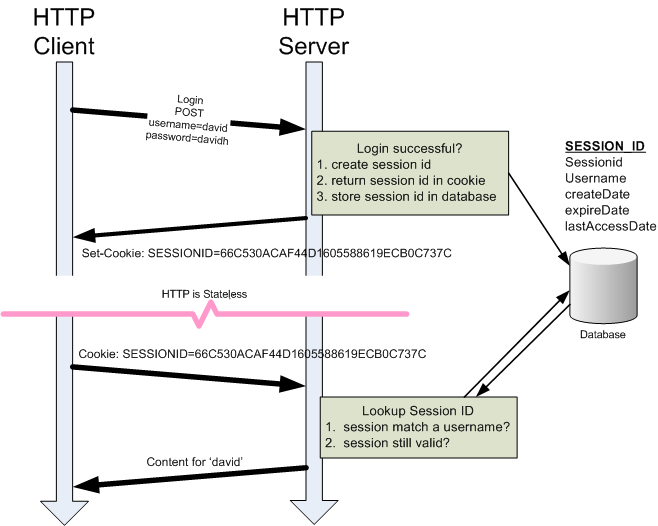
\includegraphics[width=\textwidth>]{sources/images/http_session_cookie_illustration.png}
\end{frame}

\include{sources/pages/http/demos}
\begin{frame}{Questions}
 \begin{center}
    {\LARGE Вопросы?}
 \end{center}
\end{frame}
\end{document}

